\documentclass{article}


\title{Forschungsarbeit}
\author{Laura Schillke, Sebastian Meidel, Mekong Lam }
\date{October 2018}

% Pakete laden 
\usepackage[utf8]{inputenc}
\usepackage{graphicx}
\usepackage[german]{babel}
\usepackage[default,osfigures,scale=0.95]{opensans}  %% Option 'sfdefault' only if the base font of the document is to be sans serif
\usepackage[T1]{fontenc}
% Verlinke Zitate
\usepackage{hyperref}
% Verlinke das Inhaltsverzeichnis
\hypersetup{linktocpage}
\usepackage{biblatex}
\usepackage{csquotes}
\usepackage{graphicx}
\addbibresource{mendeley_v3.bib}


%Dokument beginnt
\begin{document}

\maketitle


\newpage

\setcounter{tocdepth}{3}
\tableofcontents 



\newpage

\section{Zusammenfassung}
Bacon ipsum dolor amet shank biltong t-bone ham, ground round pastrami boudin porchetta cow fatback turkey pork tenderloin salami. Buffalo meatloaf ham hock alcatra. Boudin ground round chicken porchetta ham. T-bone spare ribs chuck fatback.

\section{Einleitung}
Bacon ipsum dolor amet shank biltong t-bone ham, ground round pastrami boudin porchetta cow fatback turkey pork tenderloin salami. Buffalo meatloaf ham hock alcatra. Boudin ground round chicken porchetta ham. T-bone spare ribs chuck fatback.

%\begin{figure}[h!]
%\centering
%
\includegraphics[scale=1.7]{universe}
%\caption{The Universe}
%\label{fig:universe}
%\end{figure}

\section{Definitionen}

\subsection{Stadt}

Haas und Neumair zufolge bezeichnet man eine Stadt als eine größere verdichtete Siedlung, die mit bestimmten Funktionen und Merkmalen charakterisiert wird \cite{HaasDefinitionWirtschaftslexikon}. Die Brockhausdefinition schreibt einer Stadt Merkmale zu wie zum Beispiel die eigene Versorgungs- und Verwaltungsstruktur, die innere Gliederung oder eine höhere Bebauungs- und Verkehrsdichte. Hinzu kommen spezielle Funktionen wie poltische Aufgaben (Haupstädte, Festungsstädte) oder wirtschaftliche Funktionen (Hansestädte, Hafenstädte, Karawanenstädte) \cite{BrockhausStadt}. Die statistischen Kriterien, die eine „Stadt“ vom „Land“ unterscheiden variieren von Land zu Land. Beispielsweise werden Städte in der Bundesrepublik Deutschland mit 
\begin{itemize}
\item 5.000 bis 20.000 Einwohnern als „Kleinstadt“,
\item 20.000 bis 50.000 Einwohnern als „Mittelstadt“,
\item ab 100.000 Einwohnern als „Großstadt“ 
\end{itemize}
bezeichnet \cite{Institutinternationaldestatistique1887BulletinStatistique}. Demgegenüber orientiert man sich in China an die Bevölkerungsdichte: 

\begin{displayquote}
In the case of cities with district establishment, the city proper refers to the whole administrative area of the district if its population density is 1 500 people per kilometre or higher [...]. \cite[S.~2]{UnitedNations2005Table2005} 
\end{displayquote}

Unabhängig von regional unterschiedlichen Kriterien lässt sich mit steigender Einwohnerzahl und -dichte einer Stadt folgern, dass auch die Anforderung an gewährleisteter Infrastruktur und Lebensmittelversorgung für die städtische Bevölkerung steigt. D.h. die Lebensmittelversorgung einer Großstadt zu gewährleisten ist schwieriger als die einer Kleinstadt. Noch größer ist die Herausforderung in Megastädten. Den Vereinten Nationen zufolge wird eine Megastadt (englisch: „Megacity“) als eine Stadt bezeichnet mit mindestens 10 Millionen Einwohnern. Im Jahr 2016 existierten 31 Megastädte und Prognosen zufolge steige die Anzahl der Megastädte im Jahr 2030 auf 41 \cite{UnitedNations2016The2016}. Tokio zählt mit 38 Millionen Einwohnern als die größte Megastadt weltweit und derzeit befinden sich die meisten Megastädte in Industrie- und Entwicklungsländern (wie in Abbildung \ref{figUrban} erkennbar). 

\begin{figure}[h]
\centering
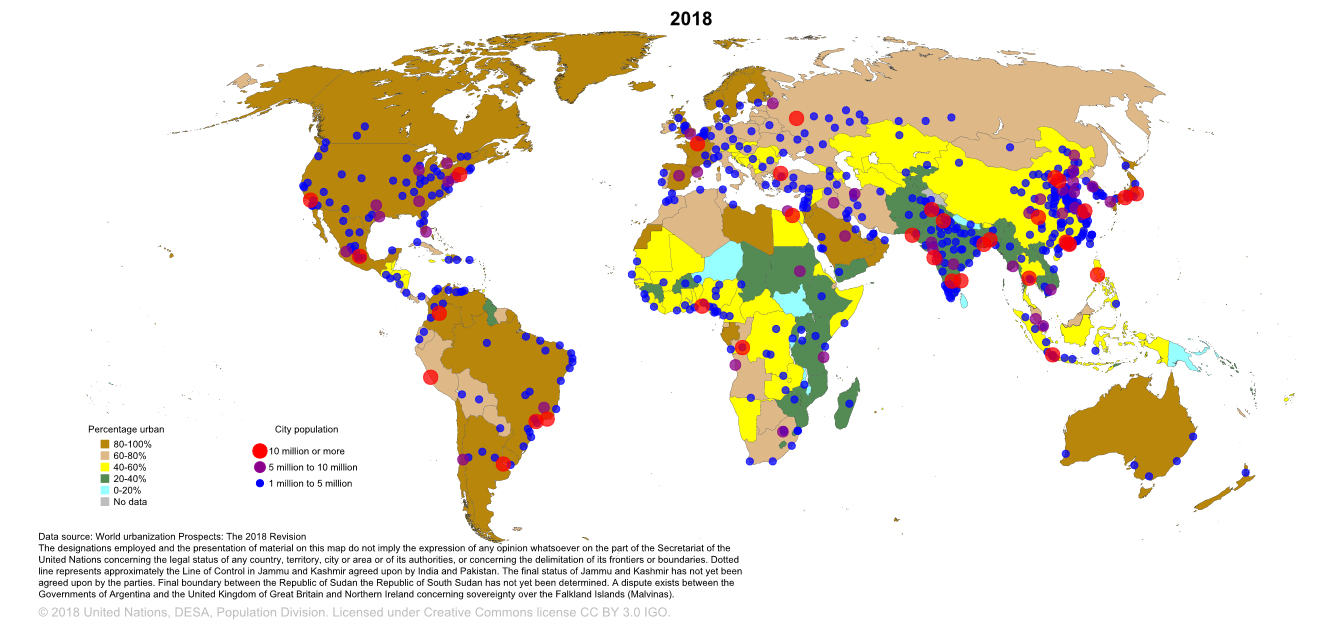
\includegraphics[width=20cm]{image_folder/CityPop_Urban.png}
\caption{Urbanisierung der Welt}
\label{figUrban}
\end{figure}

In der obigen Abbildung erkennt man, dass Nord- und Südamerika sowie Europa deutlich verstädtert sind, wohingegen viele Regionen in Afrika und Asien mehr ländliche Gebiete beinhalten. Wie gut wiederum die Lebensmittelversorgung und Infrastruktur in Megastädten ist, hängt von Megastadt zu Megastadt ab. Die Abbildung \ref{figUrbanRf} zeigt eine gute Übersicht der unterschiedlichen Verhältnisse. In dieser Forschungsarbeit der Stadtbegriff im Bezug zu ihrer fähigen Lebensmittelversorgung und Nachhaltigkeit betrachtet.


\begin{figure}[h]
\centering
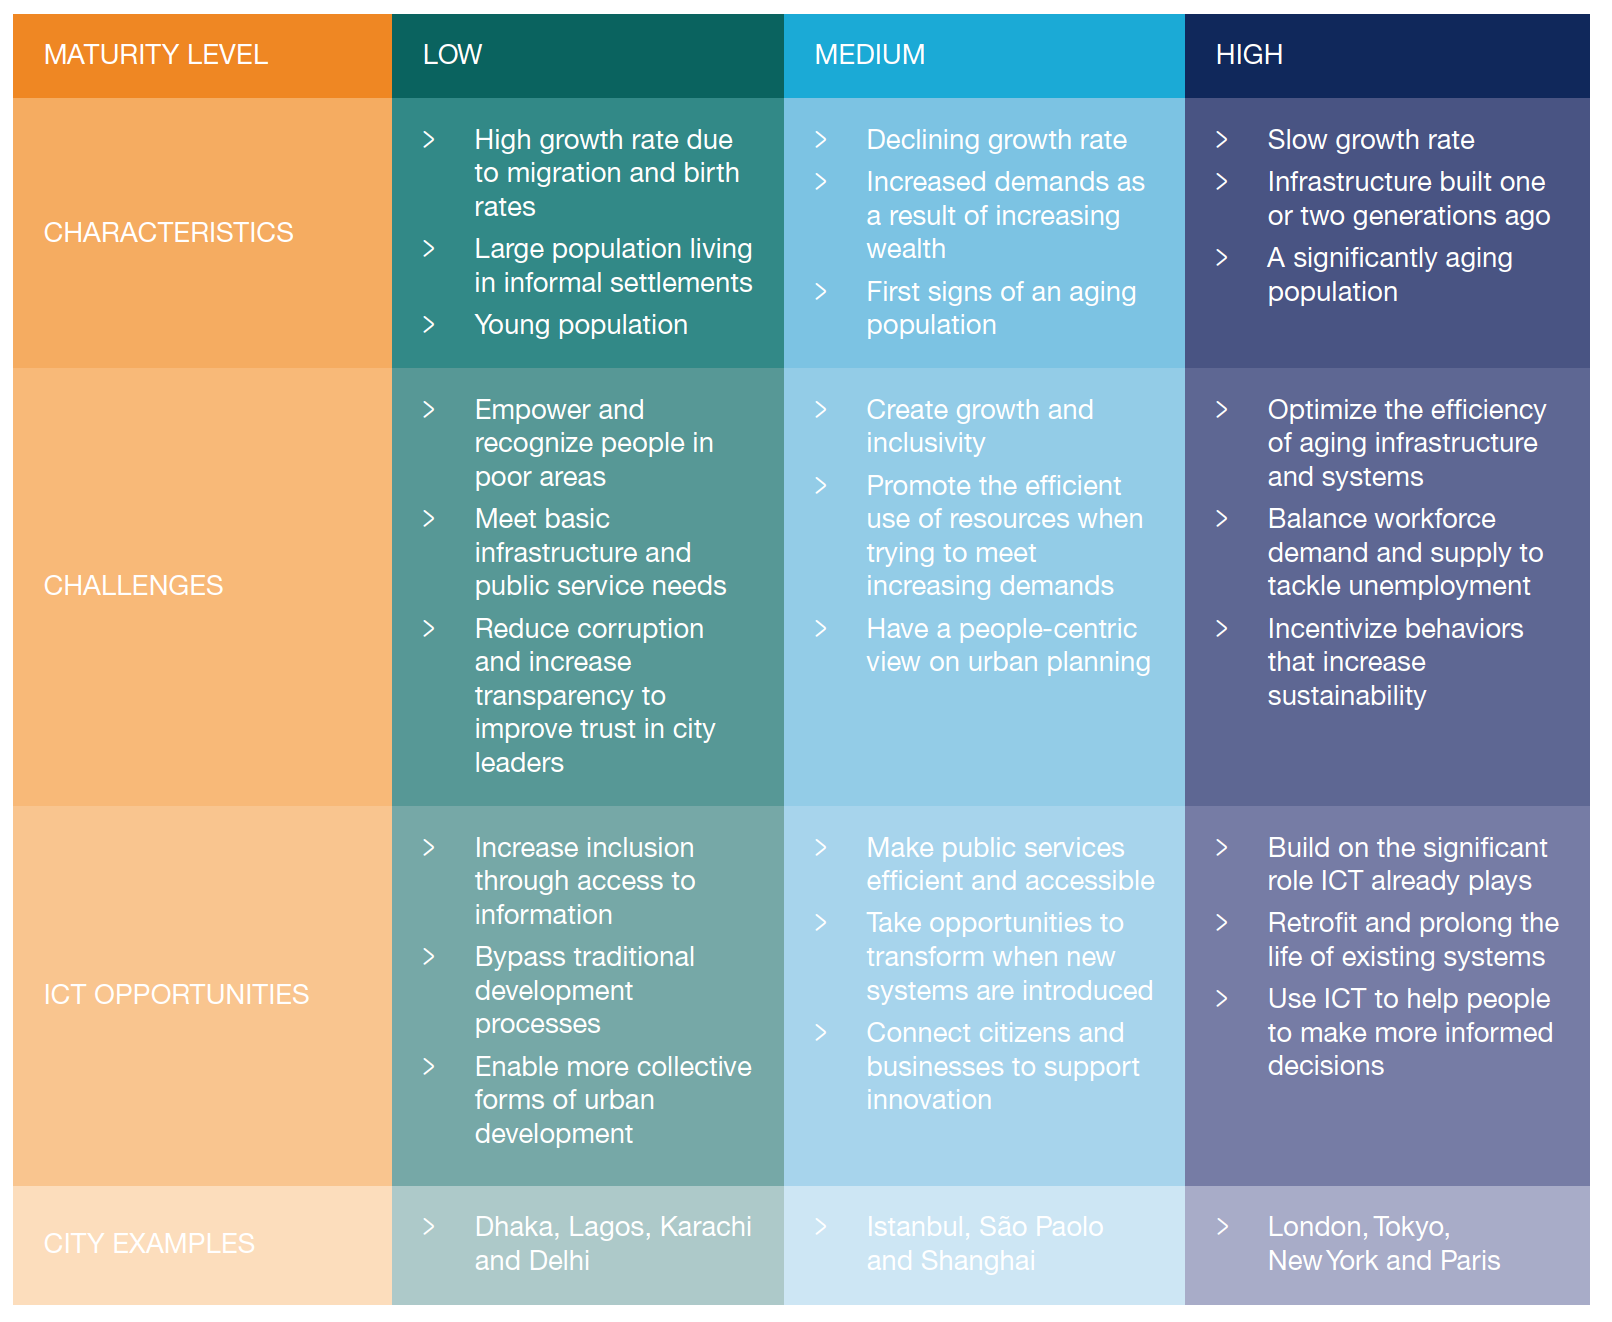
\includegraphics[width=10cm]{image_folder/urban_reifegrad.png}
\caption{Reifegrad von Megastädten}
\label{figUrbanRf}
\end{figure}

\subsubsection{Stadtökosysteme}
Stadtökosysteme sind Ökosysteme, die von Menschen erzeugt und beeinflusst werden. Wesentliche Merkmale eines Stadtökosystems sind der hohe Anteil an bebauter und versiegelter Fläche und eine hohe Bevölkerungsdichte. Genauer gesagt führt diese hohe Dichte an verschiedenen Landnutzungen dazu, dass natürlichen Ressourcen wie Wasser, Luft, Boden und Biodiversität extrem beansprucht werden. Desweiteren lässt sich über Stadtökosysteme sagen, dass ihr Erhalt von der externen Einfuhr an Lebensmitteln und Ressourcen abhängig ist  \cite[S.61]{BreusteStadtokosystemeEntwicklung}.


\subsection{Nachhaltigkeit}

Der Begriff Nachhaltigkeit ansich ist ein vielschichtiger Begriff. Er findet Verwendung in der Wirtschaft, Ökonomie, Ethik und Ökologie. So kann Nachhaltigkeit als Art und Weise des Wirtschaftens bezeichnet, „bei welcher derzeitige Bedürfnisse befriedigt werden, ohne zukünftigen Generationen die Lebensgrundlagen zu entziehen (Sustainable Development). \cite{DefinitionWirtschaftslexikonb}. Ebenso kann der Begriff als Brücke zwischen ökologischen und ökonomischen Interessen gesehen werden. Seinen Ursprung hat das Prinzip der Nachhaltigkeit in der Forstwirtschaft des 18. Jahrhunderts. Nach einer Übernutzung der Wälder und daraus resultierend knapper werdenden Holzbeständen, wurde mit Nachhaltigkeit ein Bewirtschaftungsprinzip gefordert, bei dem regenerativ gearbeitet werden sollte, das heißt “nicht mehr Holz geschlagen werden als nachwächst.“\cite{NachhaltigeBrockhaus.de}
Ab dem 19. Jahrhundert wurde zu dieser rein ressourcenökonomischen Betrachtungsweise von Nachhaltigkeit eine Umfassendere hinzugefügt, die sämtliche Funktionen des Waldes in Betracht zieht.

politische Umsetzung Nachhaltigkeit
Ergebnisse des Gipfels von Rio zur Nachhaltigkeit

\subsubsection{Kritik am Begriff der nachhaltigen Entwicklung}\cite{NachhaltigeBrockhaus.de}


Der Begriff Nachhaltigkeit kann in stark und schwach eingeteilt werden.\cite{Nachhaltigkeit}


\begin{itemize}
\item starke Nachhaltigkeit: Erhaltung der natürlichen Ressourcen steht im Vordergrund.Es beruht auf der Annahme, dass Naturgut nicht durch andere Kapitalformen ersetzt werden kann,
\item schwache Nachhaltigkeit beruht auf der Annahme das Kapital- oder Naturgut durch andere Kapitalformen erstz werden kann.
\end{itemize}
Konfliktpotenzial zwischen den Vertretern jeweiliger Positionen treten vor allem bei der Frage auf, "wie heute verursachte, aber zukünftig auftretende Umweltschäden beziehungsweise Ressourcenknappheiten zu bewerten sind.\cite{NachhaltigeBrockhaus.de}

\subsubsection{Ökologische Nachhaltigkeit}
„Die ökologische Nachhaltigkeit bezieht sich allgemein auf das Überleben und den Gesundheitszustand von Ökosystemen.“ \cite{DefinitionWirtschaftslexikonc}  Sie bezeichnet einen weitsichtiger und rücksichtsvoller Umgang mit natürlichen Ressourcen. Sofern die ökologische Nachhaltigkeit vernachlässigt wird, kann dies dazu führen, dass bestimmte Ressourcen unbrauchbar oder unwiderruflich zerstört werden mit dem Ergebnis, dass auf diese Weise jegliche weitere Entwicklungen unmöglich werden. Laut Berding und Bukow in :Die kompakte Stadt der Zukunft Auf dem Weg zu einer inklusiven und nachhaltigen Stadtgesellschaft (s.95) \cite{BerdingWolf-DietrichBukowKarinCudakHrsgDieStadtgesellschaft} gewinnt das Thema Nachhaltigkeit für die Stadtentwicklung an Wichtigkeit. 

\subsubsection{Nachhaltige Entwicklung}
 Dieser Begriff wurde von N. abgeleitet. In der internationaler Politik und bei gesellschaftlichen Bewegungen wird er als Leitbild eingesetzt. Ziel der Nachhaltigen Entwicklung ist eine dauerhalfte und gerechten Bewirtschaftung der Erde. \cite{NachhaltigeBrockhaus.de} In der Agrar- und Ernährungswirtschaft zielt der Begriff auf eine " dauerhafte Nutzung von Ressourcen bei gleichbleibender bzw. wachsender Effektivität". \cite{oppenhauser2010nachhaltigkeit} Im internationalen Sprachraum hat sich der Begriff Sustainable Development als Definition dieses Leitbild gefestigt.
 
 Konkrete Umsetzungsmethoden von Nachhaltiger Entwicklung stellen in Entwicklungsländern hauptsächlich Entwicklungsaspekte in den Vordergrund, in den industrialisierten Ländern geht es um den langfristigen Schutz und Erhalt der natürlichen Lebensgrundlage. 
\subsubsection{Ökoeffizienz}
 Der World Business Council of Sustainable Development (WBCSD) hat " für Ökoeffizienz die folgenden Kriterien erstellt: die Bereitstellung wettbewerbsfähiger Produkte, die menschliche Bedürfnisse befriedigen, die Lebensqualität fördern und dabei die Umweltauswirkungen und Ressourcenintensität während des gesamten Produktlebens minimieren." \cite{OkoeffizienzBrockhaus.de}

\begin{figure}[htp]
\centering
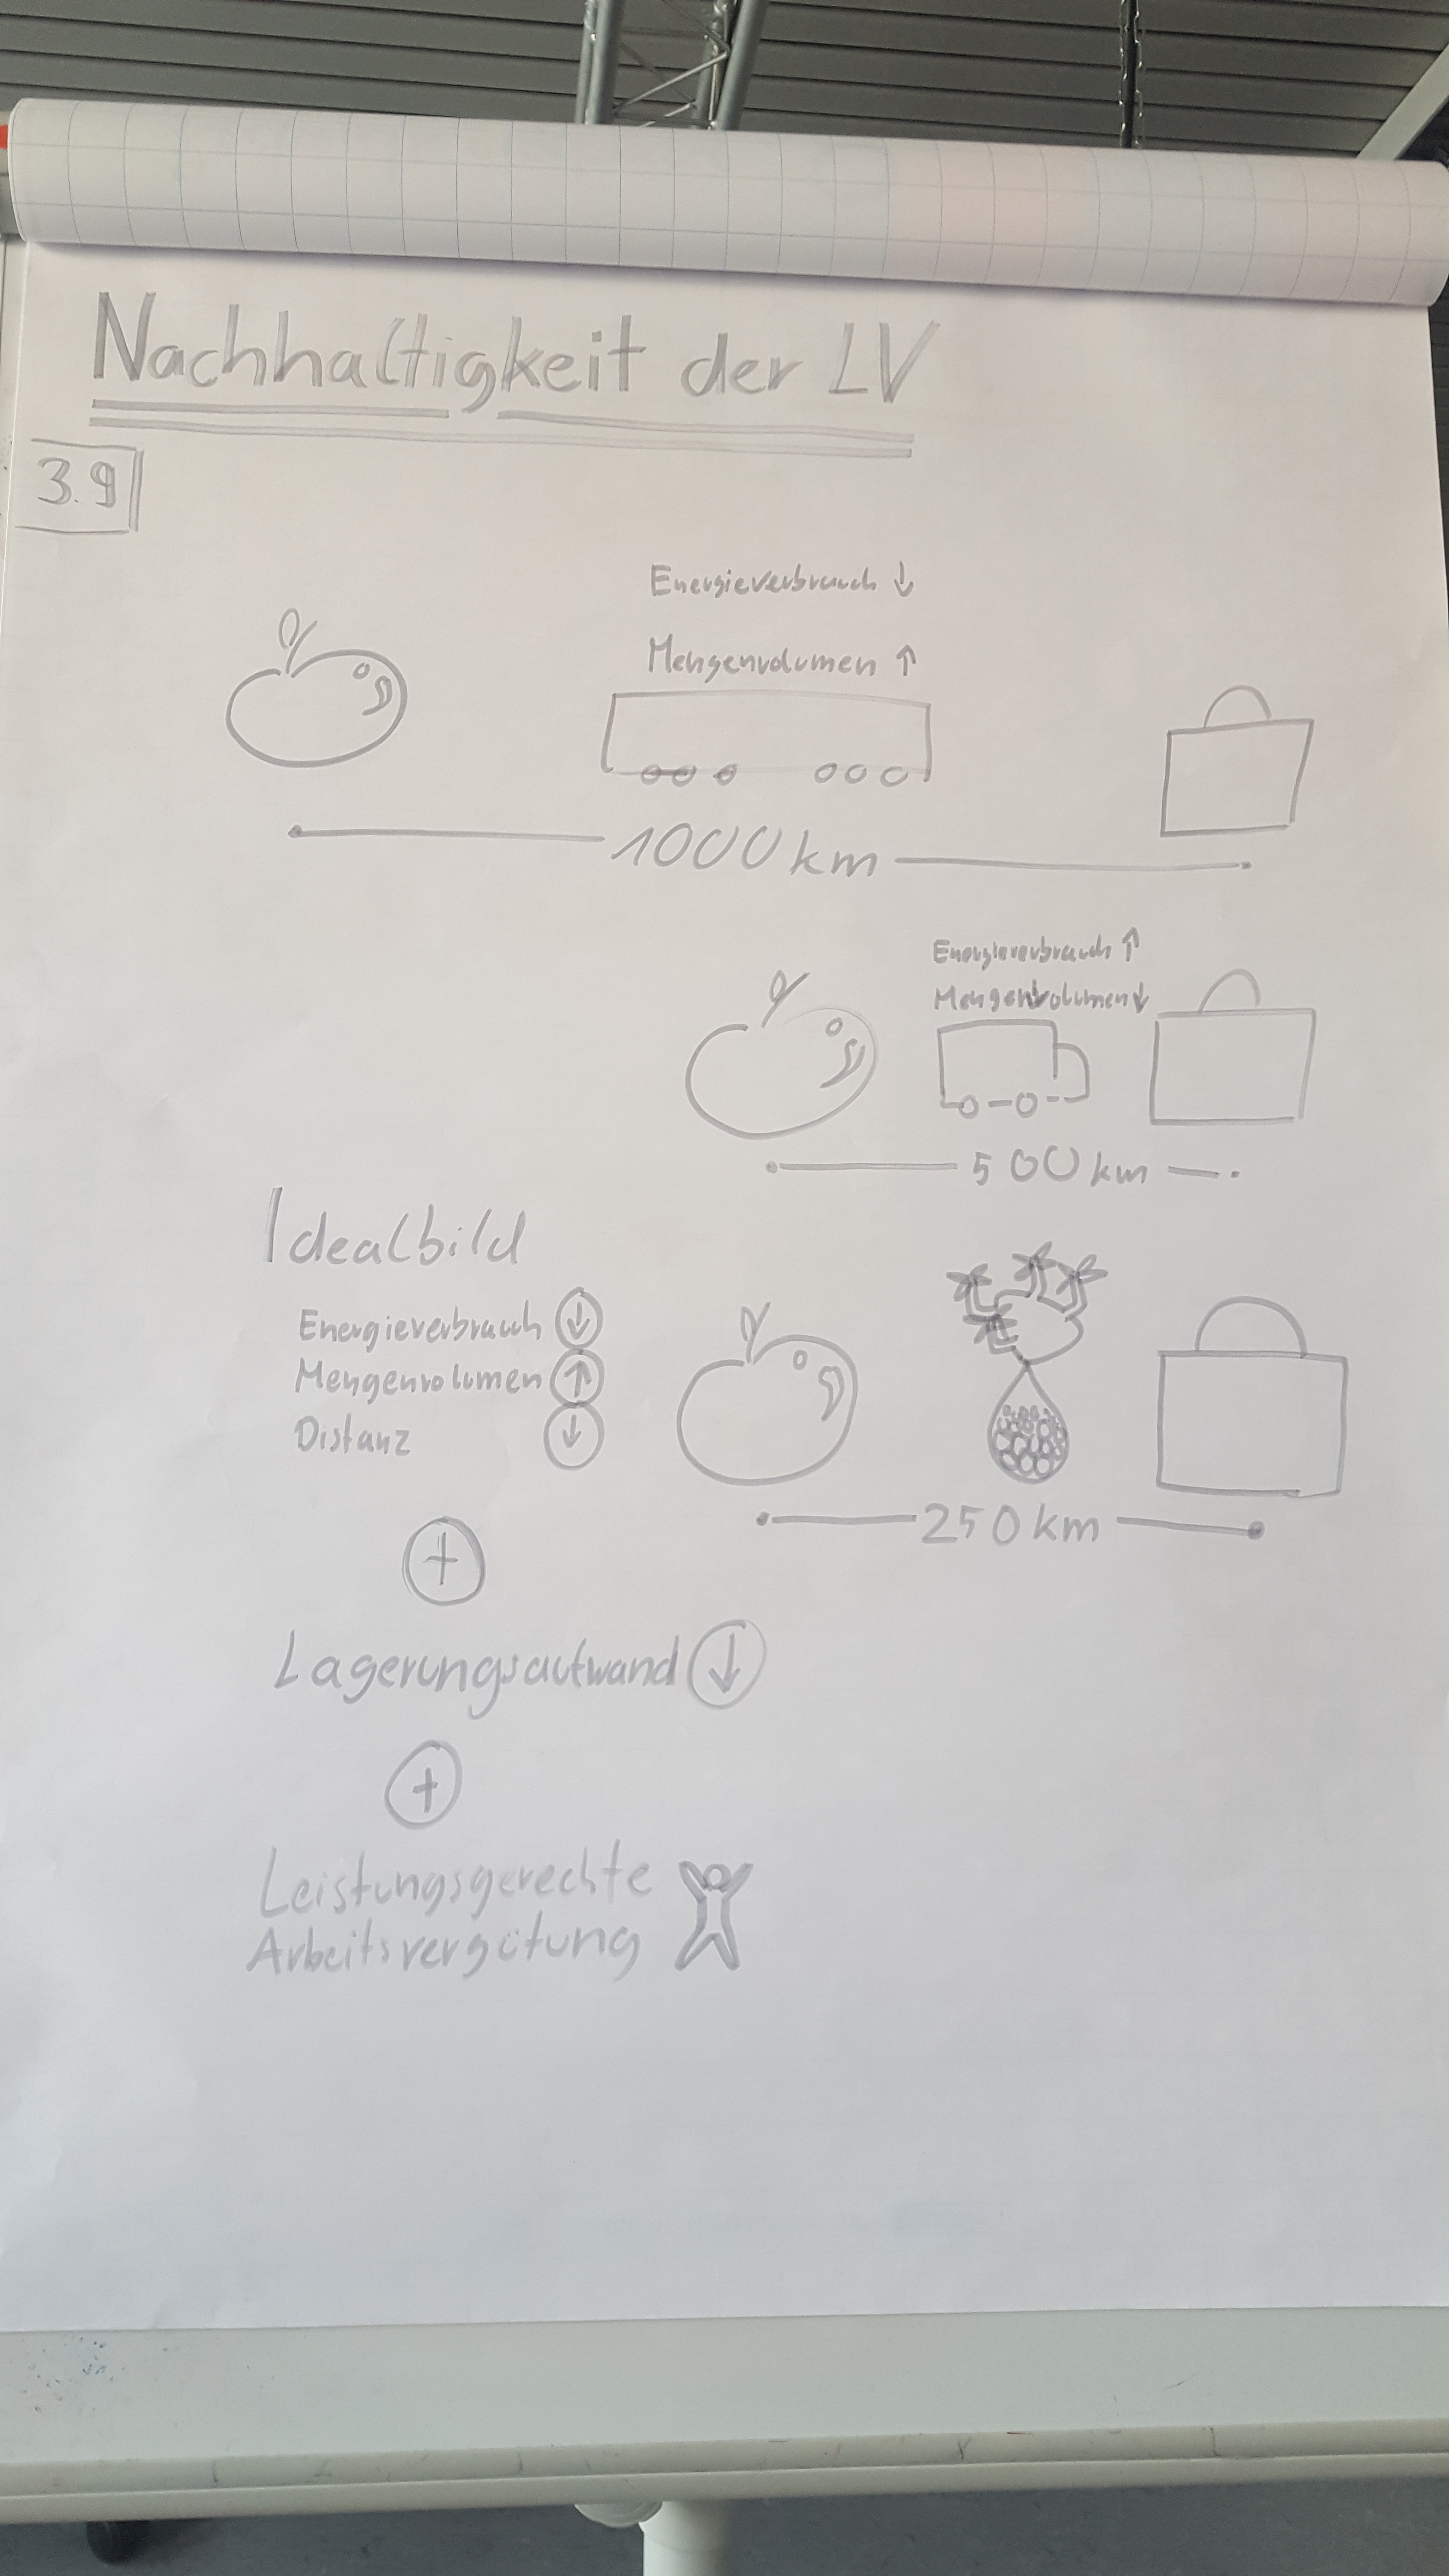
\includegraphics[width=5cm]{image_folder/skizze1.jpg}
\caption{Nachhaltigkeit der LV}
\label{fig:Skizze_Nachhaltigkeit}
\end{figure}

\newpage
\listoffigures
\printbibliography
\end{document}
